\section{Использование фреймворков для анализа программ} % (fold)

Так как сложность и количество разрабатываемых программных систем постоянно
растет, то для поддержания требуемого уровня качества все чаще начинают
использоваться специализированные инструментальные средства (фреймворки). Данные
средства поддерживают широкий набор инструментов для проведения анализа:

\begin{itemize}
    \item Построение метрик.
    \item Построение моделей программ и применение различных алгоритмов над
    этими моделями.
    \item Интерактивная визуализация процесса анализа.
\end{itemize}

\subsection{Структура фреймворков для анализа программ} % (fold)

Обычно фреймворки строятся по модульному принципу и позволяют пользователю
комбинировать используемые подходы, а также добавлять свои собственные.

На рис~\ref{fig:framework_structure} изображена типичная упрощенная структура
таких фреймворков:

\begin{figure}[h!]
    \begin{center}
        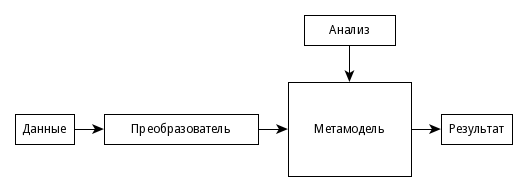
\includegraphics[width=0.7\textwidth]{img/framework_structure.png}
    \end{center}
    \caption{Упрощенная структура фреймворка для анализа программ}
    \label{fig:framework_structure}
\end{figure}

\begin{enumerate}

    \item Входными данными могут являться исходный код анализируемой программы
    или какие-то метаданные, описывающие программную систему.

    \item Преобразователь позволяет привести входные данные к виду, удобному для
    проведения дальнейшего анализа. Эта часть фреймворка является расширяемой -
    пользователь может подключать различные преобразователи для анализа
    соответствующих видов входных данных.

    \item Метамодель является промежуточным представлением анализируемой системы.
    Метамодель должна обладать следующими свойствами:

    \begin{itemize}
        \item Быть независимой от какого-либо языка программирования.
        \item Обладать необходимой полнотой представления для проведения
        различных видов анализа.
        \item Содержать обратную связь с исходными входными данными.
    \end{itemize}

    Метамодели могут поддерживать несколько парадигм программирования,
    однако чаще всего встречаются метамодели, поддерживающие
    только объектно-ориентированное программирование.

    \item После построения метамодели пользователь может использовать ее для
    проведения интересующих его видов анализа. Причем алгоритмы анализа могут
    как входить в состав реализации фреймворка, так и подключаться извне.

    \item Результаты анализа обычно предоставляются в графической или текстовой
    форме.
\end{enumerate}

\subsection{Анализ существующих решений} % (fold)
\subsubsection{SMILE} % (fold)

SMILE - фреймворк для построения метрик программных систем и обладает следующими
характеристиками:

\begin{enumerate}
    \item Независим от языка программирования, на котором написана анализируемая
    система.
    \item Поддерживает большое количество метрик.
    \item Поддерживает анализ различных версий анализируемой системы.
\end{enumerate}

В качестве метамодели SMILE использует представление в виде eCST (enriched
Concrete Syntax Tree), которая представляет собой дерево разбора программы с
добавлением универсальных узлов, что позволяет сделать дерево разбора
независимым от входного языка программирования.

На рис~\ref{fig:smile_arch} изображена архитектура данного фреймворка:

\begin{figure}[h!]
    \begin{center}
        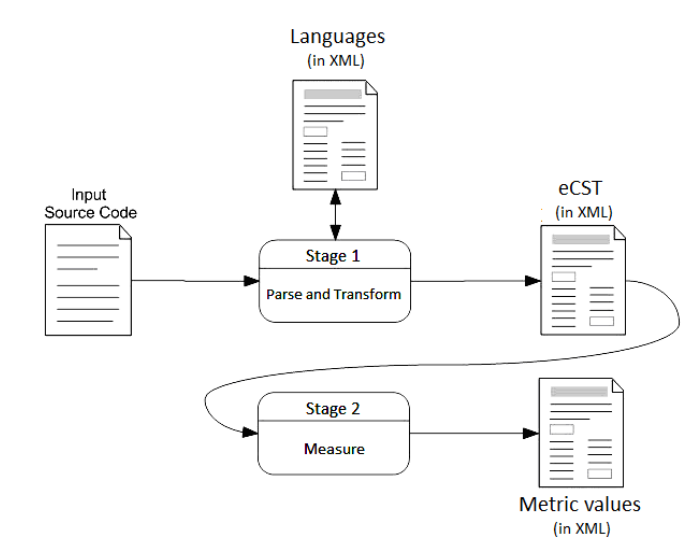
\includegraphics[width=0.6\textwidth]{img/smile_arch.png}
    \end{center}
    \caption{Архитектура фреймворка SMILE}
    \label{fig:smile_arch}
\end{figure}

\newpage
Анализ программы происходит в две фазы:

\begin{enumerate}
    \item Фаза 1
    \begin{itemize}
        \item Определение языка программирования, на котором написана
        анализируемая программа.
        \item Вызов парсера этого языка для построения CST и преобразование в
        eCST.
        \item Вывод результата в формате XML.
    \end{itemize}

    \item Фаза 2
    \begin{itemize}
        \item Считывание eCST из файла.
        \item Подсчет метрик.
        \item Сохранение результата в формате XML.
    \end{itemize}
\end{enumerate}

На данный момент фреймворк находится на стадии разработки и поддерживает
малое количество метрик и языков программирования.

\subsubsection{Moose} % (fold)

Moose является платформой для анализа программ и поддерживает большое количество
различных видов анализа:

\begin{enumerate}
    \item Построение и визуализация метрик.
    \item Обнаружение клонов.
    \item Построение графа зависимостей между пакетами.
    \item Вывод словаря, используемого в проекте.
    \item Поддержка браузеров исходного кода.
\end{enumerate}

Moose использует целое семейство метамоделей под названием FAMIX. Данное
семейство обладает довольно сложной структурой, упрощенная вид которой приведен
на рис~\ref{fig:famix_hierarchy}

\begin{figure}[h!]
     \begin{center}
         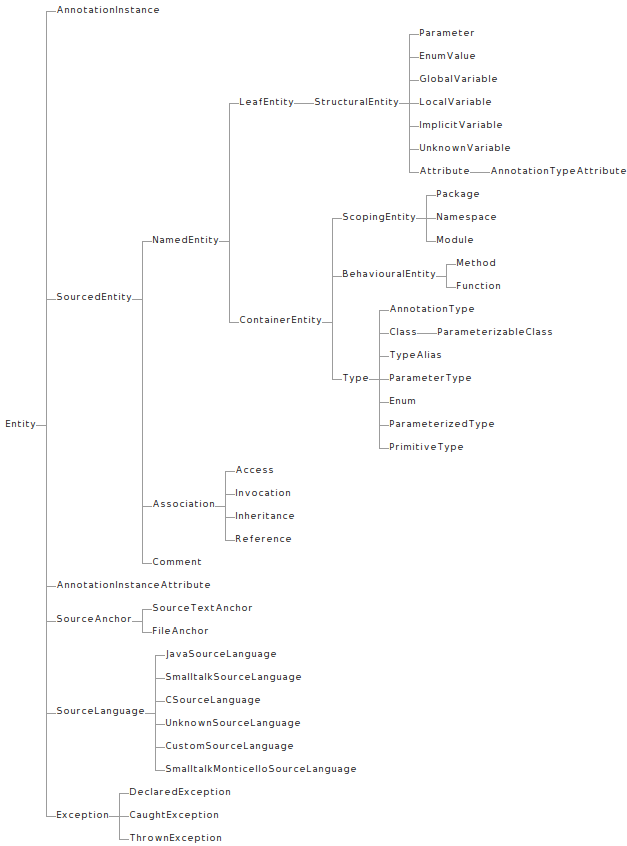
\includegraphics[width=0.9\textwidth]{img/famix_hierarchy.png}
     \end{center}
     \caption{Структура метамоделей семейства FAMIX}
     \label{fig:famix_hierarchy}
 \end{figure}

\newpage
Анализ программы происходит следующим образом:

\begin{enumerate}
    \item Импортирование входных данных. Импортирование может происходить как
    при помощи встроенных средств (Moose поддерживает Smalltalk, XML и MSE),
    так и при помощи сторонних средств.
    \item После импортирования данные приводятся к одной из метамоделей
    семейства FAMIX.
    \item Применение заданных алгоритмов анализа.
\end{enumerate}

Архитектура фреймворка приведена на рис~\ref{fig:moose_architecture}

\begin{figure}[h!]
    \begin{center}
        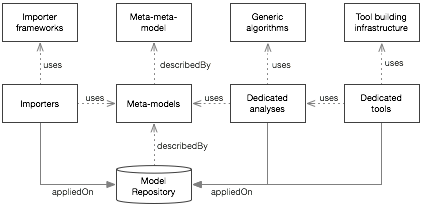
\includegraphics[]{img/moose_architecture.png}
    \end{center}
    \caption{Архитектура фреймворка Moose}
    \label{fig:moose_architecture}
\end{figure}

Разработка Moose активно ведется с 1996 года и на данный момент этот фреймворк
является одним из самых совершенных средств для анализа программ.

\subsubsection{LLVM} % (fold)

LLVM - фреймворк для анализа и трансформации программ, путем предоставления
информации для трансформаций компилятору во время компиляции, линковки и
исполнения.

LLVM использует промежуточное представление, в основе которого лежит
представление в виде SSA. Промежуточное представление является набором
RISC-подобных команд и содержит дополнительную информацию более высокого уровня,
например информацию о типах и графе потока управления.

Фреймворк обладает следующими особенностями:

\begin{enumerate}
    \item Сохранение информации о программе даже во время исполнения и между
    запусками.
    \item Предоставление информации пользователю для профилирования и
    оптимизации.
    \item Промежуточное представление не зависит от языка программирования.
    \item Возможность оптимизации всей системы в целом (после этапа линковки).
\end{enumerate}

Архитектура LLVM приведена на рис~\ref{fig:llvm_arch}

\begin{figure}[h!]
    \begin{center}
        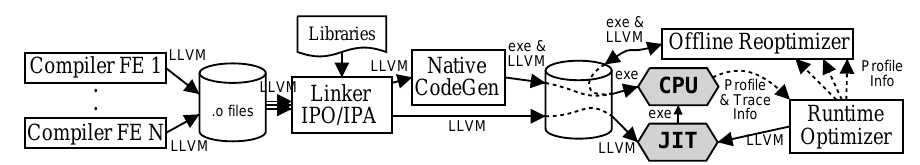
\includegraphics[width=\textwidth]{img/llvm_arch.png}
    \end{center}
    \caption{Архитектура LLVM}
    \label{fig:llvm_arch}
\end{figure}

Front-end компиляторы транслируют исходную программу в промежуточное
представление LLVM, которое затем компонуется LLVM-линкером. На этой стадии
может проводиться межпроцедурный анализ. Получившийся код затем транслируется
в машинный код для целевой платформы.
